\documentclass[letterpaper,11pt,twoside]{article}
\usepackage{graphicx} % Required for inserting images
\usepackage[table,xcdraw,dvipsnames]{xcolor}
\usepackage{amsmath,amsfonts,amssymb,amsthm}
\usepackage{listings}
\usepackage{lipsum}
\usepackage{hyperref}
\usepackage{mathrsfs}
\usepackage{tikz}
\usepackage{mathtools}
\usetikzlibrary{arrows.meta}
\usepackage{enumitem}

\usepackage{tikz}
\usepackage[siunitx, RPvoltages]{circuitikz}
\usetikzlibrary{3d}
\usepackage{comment}
\usepackage{caption,subcaption}
\usepackage{pgfplots}
\pgfplotsset{compat=newest} % or a newer version if available
\usepgfplotslibrary{groupplots}
\usetikzlibrary{pgfplots.groupplots}
\usetikzlibrary{shapes.geometric, arrows}
\tikzstyle{arrow} = [->,>=stealth,shorten >=2pt]
\newcommand{\ket}[1]{|#1\rangle}
\newcommand{\bra}[1]{\langle#1|}
\newcommand{\br}{\bm{r}}
\newcommand{\bR}{\bm{R}}
\newcommand{\bp}{\bm{p}}
\newcommand{\bP}{\bm{P}}
\newcommand{\braket}[1]{\langle#1\rangle}
\newcommand{\F}{\mathscr{F}}
\newcommand{\E}{\mathscr{E}}
\newcommand{\re}[1]{\text{Re}\left(#1\right)}
\newcommand{\im}[1]{\text{Im}\left(#1\right)}
\usepackage{dsfont}
\usepackage{cancel}
\usepackage{bm}
\usepackage{fancyhdr}
\usepackage[utf8x]{inputenc}
\usepackage[T1]{fontenc}
\usepackage[margin=0.8in,top=1in,bottom=1in]{geometry}
\newcommand{\hn}{\bm{\hat{n}}}
\newcommand{\hr}{\bm{\hat{r}}}
\newcommand{\hx}{\bm{\hat{x}}}
\newcommand{\hy}{\bm{\hat{y}}}
\newcommand{\hz}{\bm{\hat{z}}}
%%%%%
\begin{filecontents*}{refs.bib}
@book{bornwolf,
  author    = {Born, M. and Wolf, E.},
  title     = {Principles of Optics},
  publisher = {Pergamon Press},
  edition   = {7},
  year      = {1999}
}
@book{hecht,
  author    = {Hecht, E.},
  title     = {Optics},
  publisher = {Addison-Wesley},
  edition   = {5},
  year      = {2016}
}
\end{filecontents*}
%
\newcommand{\institution}{University of Arizona}
\newcommand{\autor}{Nicolás Hernández Alegría}
\newcommand{\course}{OPTI 570 Quantum Mechanics}
\newcommand{\assignment}{Assignment 9}
%
\title{\textbf{\assignment}\\\course\\{\Large\institution}}
\author{\autor}
\date{\today\\Total time: 8 hours}
%
\renewcommand{\sectionmark}[1]{\markright{#1}}
\fancypagestyle{mainstyle}{
    \fancyhf{} % Clear all header and footer fields
    \fancyfoot[C]{\thepage}
    \fancyhead[LE,RO]{\course} % Section name on odd pages
    \fancyhead[LO,RE]{\assignment}
    % Optional: Thin rules
    \renewcommand{\headrulewidth}{0pt} % Header rule
    \renewcommand{\footrulewidth}{0pt} % No footer rule
}
%
\begin{document}

\pagestyle{mainstyle}
\maketitle
%%
\section*{Problem I}
\begin{enumerate}[itemsep=0pt,topsep=0pt,label=\alph*)]
  \item The general expression for the transition probability is:
  \begin{align*}
    P_{\ket{+}\to\ket{-}}(t)=\left|\frac{\Omega_0}{\Omega}\right|^2\sin^2\frac{\Omega t}{2},\quad \Omega=\sqrt{\Omega_0^2+\Delta^2}.
  \end{align*}
  By evaluating the different detuning given, we have:
  \begin{align*}
    \Delta=0:&\qquad \Omega=\Omega_0\Longrightarrow P_{\ket{+}\to\ket{-}}(t)=\sin^2\frac{\Omega_0t}{2}\\
    \Delta=|\Omega_0|:&\qquad \Omega=\sqrt{2}\Omega_0\Longrightarrow P_{\ket{+}\to\ket{-}}(t)=\frac{1}{2}\sin^2\frac{\sqrt{2}\Omega_0t}{2}\\
    \Delta=2|\Omega_0|:&\qquad \Omega=\sqrt{5}\Omega_0\Longrightarrow P_{\ket{+}\to\ket{-}}(t)=\frac{1}{5}\sin^2\frac{\sqrt{5}\Omega_0t}{2}
  \end{align*}
  For visualization, we will set $\Omega_0=1$.
  \begin{figure}[h!]
    \centering
    \begin{circuitikz}[xscale=1,yscale=2,scale=.6]
      \def\Omo{1}
      \draw[arrow](0,0)--({6*pi/\Omo+1},0)node[below]{$t$};
      \draw[arrow](0,0)--(0,2)node[right]{$f(t)$};
      \draw[very thick,OliveGreen,domain=0:{6*pi/\Omo},samples=500] plot(\x,{ ( sin( deg(\Omo*\x/2) ) )^2 });
      \draw[very thick,Black,domain=0:{6*pi/\Omo},samples=500] plot(\x,{ (1/2)*( sin( deg(sqrt(2)*\Omo*\x/2) ) )^2 });
      \draw[very thick,NavyBlue,domain=0:{6*pi/\Omo},samples=500] plot(\x,{ (1/5)*( sin( deg(sqrt(5)*\Omo*\x/2) ) )^2 });
      \foreach \x in {1,...,6}{\draw({\x*pi/\Omo},.1)--({\x*pi/\Omo},-.1)node[below]{$\frac{\x\pi}{|\Omega_0|}$}; }
      \foreach \y in {1,1/2,1/5}{\draw(.1,\y)--(-.1,\y)node[left]{\small$\y$};}
      \begin{scope}[shift={(21,1)}] % move legend to top-right
          \draw[very thick,OliveGreen](0,0)--(0.8,0)node[right,black]{$\Delta=0$};
          \draw[very thick,Black](0,-0.5)--(0.8,-0.5)node[right,black]{$\Delta=|\Omega_0|$};
          \draw[very thick,NavyBlue](0,-1)--(0.8,-1)node[right,black]{$\Delta=2|\Omega_0|$};
      \end{scope}
    \end{circuitikz}
  \end{figure}
  \item The Hamiltonian can be written in term of the Pauli matrices when $\Omega_0=|\Omega_0|e^{i\beta}$:
  \begin{align*}
    H=\frac{\hbar}{2}[\Delta\sigma_z+|\Omega_0|\cos\beta\sigma_x-|\Omega_0|\sin\beta\sigma_y]=\frac{\hbar}{2}\bm{\Omega}\cdot\bm{\sigma}.
  \end{align*}
  The last is called effective field, or Rabi vector.
  The Bloch sphere is $\br(t)=\braket{\psi(t)|\bm{\sigma}|\psi(t)}$, with $\bR(0)=(0,0,1)$.
  \begin{figure}[h!]
    \centering
    \begin{subfigure}{.3\columnwidth}
      \centering
      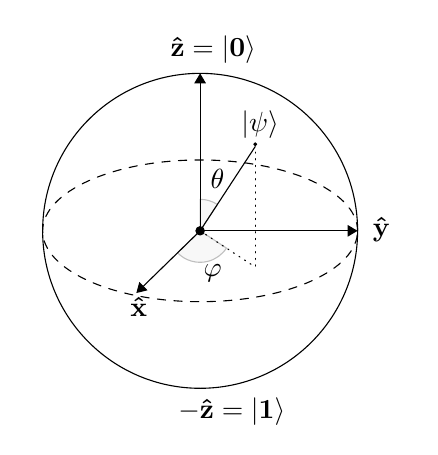
\begin{tikzpicture}[line cap=round, line join=round, >=Triangle]
      \clip(-2.19,-2.49) rectangle (2.66,2.58);
      \draw [shift={(0,0)}, lightgray, fill, fill opacity=0.1] (0,0) -- (56.7:0.4) arc (56.7:90.:0.4) -- cycle;
      \draw [shift={(0,0)}, lightgray, fill, fill opacity=0.1] (0,0) -- (-135.7:0.4) arc (-135.7:-33.2:0.4) -- cycle;
      \draw(0,0) circle (2cm);
      \draw [rotate around={0.:(0.,0.)},dash pattern=on 3pt off 3pt] (0,0) ellipse (2cm and 0.9cm);
      \draw (0,0)-- (0.70,1.07);
      \draw [->] (0,0) -- (0,2);
      \draw [->] (0,0) -- (-0.81,-0.79);
      \draw [->] (0,0) -- (2,0);
      \draw [dotted] (0.7,1)-- (0.7,-0.46);
      \draw [dotted] (0,0)-- (0.7,-0.46);
      \draw (-0.08,-0.3) node[anchor=north west] {$\varphi$};
      \draw (0.01,0.9) node[anchor=north west] {$\theta$};
      \draw (-1.01,-0.72) node[anchor=north west] {$\mathbf {\hat{x}}$};
      \draw (2.07,0.3) node[anchor=north west] {$\mathbf {\hat{y}}$};
      \draw (-0.5,2.6) node[anchor=north west] {$\mathbf {\hat{z}=|0\rangle}$};
      \draw (-0.4,-2) node[anchor=north west] {$-\mathbf {\hat{z}=|1\rangle}$};
      \draw (0.4,1.65) node[anchor=north west] {$|\psi\rangle$};
      \scriptsize
      \draw [fill] (0,0) circle (1.5pt);
      \draw [fill] (0.7,1.1) circle (0.5pt);
    \end{tikzpicture}
    \caption{$\Delta=0$}
    \end{subfigure}
    \hfill
    \begin{subfigure}{.3\columnwidth}
      \centering
      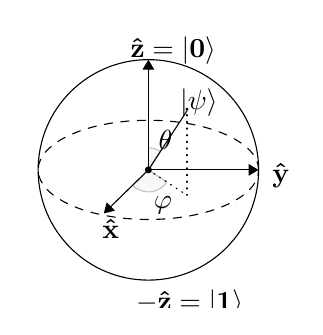
\begin{tikzpicture}[line cap=round, line join=round, >=Triangle,scale=.7]
      \clip(-2.19,-2.49) rectangle (2.66,2.58);
      \draw [shift={(0,0)}, lightgray, fill, fill opacity=0.1] (0,0) -- (56.7:0.4) arc (56.7:90.:0.4) -- cycle;
      \draw [shift={(0,0)}, lightgray, fill, fill opacity=0.1] (0,0) -- (-135.7:0.4) arc (-135.7:-33.2:0.4) -- cycle;
      \draw(0,0) circle (2cm);
      \draw [rotate around={0.:(0.,0.)},dash pattern=on 3pt off 3pt] (0,0) ellipse (2cm and 0.9cm);
      \draw (0,0)-- (0.70,1.07);
      \draw [->] (0,0) -- (0,2);
      \draw [->] (0,0) -- (-0.81,-0.79);
      \draw [->] (0,0) -- (2,0);
      \draw [dotted] (0.7,1)-- (0.7,-0.46);
      \draw [dotted] (0,0)-- (0.7,-0.46);
      \draw (-0.08,-0.3) node[anchor=north west] {$\varphi$};
      \draw (0.01,0.9) node[anchor=north west] {$\theta$};
      \draw (-1.01,-0.72) node[anchor=north west] {$\mathbf {\hat{x}}$};
      \draw (2.07,0.3) node[anchor=north west] {$\mathbf {\hat{y}}$};
      \draw (-0.5,2.6) node[anchor=north west] {$\mathbf {\hat{z}=|0\rangle}$};
      \draw (-0.4,-2) node[anchor=north west] {$-\mathbf {\hat{z}=|1\rangle}$};
      \draw (0.4,1.65) node[anchor=north west] {$|\psi\rangle$};
      \scriptsize
      \draw [fill] (0,0) circle (1.5pt);
      \draw [fill] (0.7,1.1) circle (0.5pt);
    \end{tikzpicture}
    \caption{$\Delta=|\Omega_0|$}
    \end{subfigure}
    \hfill
    \begin{subfigure}{.3\columnwidth}
      \centering
      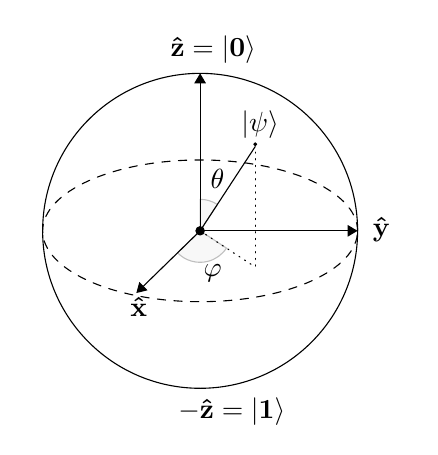
\begin{tikzpicture}[line cap=round, line join=round, >=Triangle]
      \clip(-2.19,-2.49) rectangle (2.66,2.58);
      \draw [shift={(0,0)}, lightgray, fill, fill opacity=0.1] (0,0) -- (56.7:0.4) arc (56.7:90.:0.4) -- cycle;
      \draw [shift={(0,0)}, lightgray, fill, fill opacity=0.1] (0,0) -- (-135.7:0.4) arc (-135.7:-33.2:0.4) -- cycle;
      \draw(0,0) circle (2cm);
      \draw [rotate around={0.:(0.,0.)},dash pattern=on 3pt off 3pt] (0,0) ellipse (2cm and 0.9cm);
      \draw (0,0)-- (0.70,1.07);
      \draw [->] (0,0) -- (0,2);
      \draw [->] (0,0) -- (-0.81,-0.79);
      \draw [->] (0,0) -- (2,0);
      \draw [dotted] (0.7,1)-- (0.7,-0.46);
      \draw [dotted] (0,0)-- (0.7,-0.46);
      \draw (-0.08,-0.3) node[anchor=north west] {$\varphi$};
      \draw (0.01,0.9) node[anchor=north west] {$\theta$};
      \draw (-1.01,-0.72) node[anchor=north west] {$\mathbf {\hat{x}}$};
      \draw (2.07,0.3) node[anchor=north west] {$\mathbf {\hat{y}}$};
      \draw (-0.5,2.6) node[anchor=north west] {$\mathbf {\hat{z}=|0\rangle}$};
      \draw (-0.4,-2) node[anchor=north west] {$-\mathbf {\hat{z}=|1\rangle}$};
      \draw (0.4,1.65) node[anchor=north west] {$|\psi\rangle$};
      \scriptsize
      \draw [fill] (0,0) circle (1.5pt);
      \draw [fill] (0.7,1.1) circle (0.5pt);
    \end{tikzpicture}
    \caption{$\Delta=2|\Omega_0|$}
    \end{subfigure}
  \end{figure}

\end{enumerate}


%%
\section*{Problem II}
\begin{enumerate}[itemsep=0pt,topsep=0pt,label=\alph*)]
  \item The unit-vector in cartesian coordinates expressed in terms of the spherical quantities is:
  \begin{align*}
    \hr=\sin\theta\cos\phi\hx+\sin\theta\sin\phi\hy+\cos\theta\hz.
  \end{align*}
  We now try to use the table given in the Field guide to substitute these coefficients and express $\hr$ in terms of the Spherical harmonics.
  The z-direction is the easiest as it only has one quantitiy involved. We now that $Y_1^0$ has cosine of that angle, so we can use it to say that:
  \begin{align*}
    Y_1^0=\sqrt{\frac{3}{4\pi}}\cos\theta\longrightarrow\cos\theta=\sqrt{\frac{4\pi}{3}}Y_1^0.
  \end{align*}
  For the x-direction, we have the term $\sin\theta\cos\phi$ meaning we need to combine some spherical to have this product form.
  Using $Y_1^{\pm1}$ we can create a cosine by considering both sign and collect the expoential:
  \begin{align*}
    Y_1^{-1}-Y_1^{1}=\sqrt{\frac{3}{8\pi}}\sin\theta\left[e^{-i\phi}+e^{i\phi}\right]=\sqrt{\frac{3}{2\pi}}\sin\theta\cos\phi\longrightarrow\sin\theta\cos\phi=\sqrt{\frac{2\pi}{3}}(Y_1^{-1}-Y_1^1).
  \end{align*}
  Similarly, we play with $Y_1^{\pm1}$ to get the $\sin\phi$ term:
  \begin{align*}
    Y_1^{-1}+Y_1^{-1}=\sqrt{\frac{3}{8\pi}}\sin\theta\left[-e^{-i\phi}+e^{i\phi}\right]=2i\sqrt{\frac{3}{8\pi}}\sin\theta\sin\phi\longrightarrow\sin\theta\sin\phi=-i\sqrt{\frac{2\pi}{3}}(Y_1^{-1}+Y_1^1).
  \end{align*}
  Therefore, we finally have 
  \begin{align*}
    \hr=\sqrt{\frac{2\pi}{3}}(Y_1^{-1}-Y_1^1)\hx-i\sqrt{\frac{2\pi}{3}}(Y_1^{-1}+Y_1^1)\hy+\sqrt{\frac{4\pi}{3}}Y_1^0\hz.
  \end{align*}
  \item We have already substituted $x$ for $\sin\theta\cos\phi$ and in terms of the spherical harmonics. The only quantity we need to compute is the $r$, which is obtained by squaring the compoents.
  \begin{align*}
    r^2&=x^2+y^2+z^2=\left[\sqrt{\frac{2\pi}{3}}(Y_1^{-1}-Y_1^1)\right]^2+\left[-i\sqrt{\frac{2\pi}{3}}(Y_1^{-1}+Y_1^1)\right]^2+\left[\sqrt{\frac{4\pi}{3}}Y_1^0\right]^2\\
    &=\frac{2\pi}{3}\left[(Y_1^{-1})^2-2Y_1^{-1}Y_1^1+(Y_1^1)^2+(Y_1^{-1})^2+2Y_1^{-1}Y_1^1+(Y_1^1)^2\right]+\frac{4\pi}{3}(Y_1^0)^2\\
    r^2&=\frac{4\pi}{3}\left[(Y_1^{-1})^2+(Y_1^1)^2+(Y_1^0)^2\right].
  \end{align*} 
  Then, we have 
  \begin{align*}
    F(x,y,z)=\frac{(Y_1^{-1}-Y_1^1-iY_1^{-1}-iY_1^1+\sqrt{2}Y_1^0)}{\sqrt{2}[(Y_1^{-1})^2+(Y_1^1)^2+(Y_1^0)^2]}.
  \end{align*}
\end{enumerate}

%%
\section*{Problem III}
The initial state is $\ket{+}_z$. The firt pulse is along the y-direction which make a Hamiltonian of the form 
\begin{align*}
  H=-\gamma\hbar/2\bm{\sigma}\cdot\bm{B}\Longrightarrow U(t)=e^{-iHt/\hbar}=e^{-i\alpha\bm{\sigma}\cdot\bm{B}/2},\quad\alpha=-|\gamma|Bt.
\end{align*}
where $\alpha$ is the rotation angle generated by the pulse along y.

%%
\section*{Problem IV}




%\nocite{*}
%\bibliographystyle{plain}   % or unsrt, alpha, apalike, etc.
%\bibliography{refs}

\end{document}
